\hypertarget{which-values-allow-records-an-exact-window}{%
\section{Which values allow records: an exact
window}\label{which-values-allow-records-an-exact-window}}

A constant term enters the expansion history, and through it the growth
of structure. This section asks a question that does not require knowing
the value: in a simple universe that forms structure, which values of
the constant allow lasting, distinguishable records? The answer is an
exact window for a declared toy model. The selection predicate never
mentions \(\lambda\).

\hypertarget{the-model}{%
\subsection{The model}\label{the-model}}

Units are chosen so that the matter density is \(\rho_m=a^{-3}\) and
\(H^2=a^{-3}+\lambda\); the swept parameter \(\lambda\) is a signed
constant. Each of \(N=64\) patches carries a linear density contrast
\(\delta_i(a)=m_i\,D_\lambda(a)\), where \(D_\lambda\) solves the
standard linear growth equation \(\ddot D+2H\dot D=\tfrac32\rho_m D\)
from \(a_0=10^{-3}\) with \(D(a_0)=1\) and \(dD/da(a_0)=1/a_0\). The
amplitudes \(m_i\) are drawn once per seed from a half-normal
distribution of scale \(10^{-3}\), and each patch carries an independent
Boolean tag. The rules are:

\begin{itemize}
\tightlist
\item
  \textbf{formation:} a patch collapses when its contrast reaches
  \(\delta_c=1.686\) \citep{GunnGott1972}, and its tag is frozen as a
  record;
\item
  \textbf{erasure:} if the expansion turns around at or before the
  horizon \(A=20\), which happens exactly when
  \(\lambda\le-A^{-3}=-1/8000\), all records are erased; this is an
  imposed rule standing in for recollapse;
\item
  \textbf{seed predicate:} a seed passes if, by \(a=A\), collapsed
  patches carrying \emph{both} tag values exist and have not been
  erased;
\item
  \textbf{aggregate gate:} a value of \(\lambda\) is admitted if at
  least 10 of the 12 seeds pass (the declared 80\% gate).
\end{itemize}

Two facts about the model drive everything below. On the expanding
branch, which exists through \(a=A\) exactly when \(\lambda>-1/8000\),
the growth factor \(D_\lambda(a)\) is strictly increasing in \(a\) and,
for every \(a>a_0\), strictly decreasing in \(\lambda\): more dark
energy means less growth. And a seed \(j\) passes exactly when
\[\lambda>-1/8000\quad\text{and}\quad G(\lambda)=D_\lambda(A)\ge T_j=\max\bigl(\delta_c/m_{j,0},\,\delta_c/m_{j,1}\bigr),\]
where \(m_{j,0}\) and \(m_{j,1}\) are the largest amplitudes carrying
each tag (with \(T_j=\infty\) if a tag is absent). The aggregate gate is
then \(\lambda>-1/8000\) and \(G(\lambda)\ge T_\star\), where
\(T_\star\) is the tenth smallest of the twelve seed thresholds.

\hypertarget{the-window}{%
\subsection{The window}\label{the-window}}

\begin{theorem}[Record window]\label{thm:window}
For the realized twelve-seed, 64-patch population, the set of admitted $\lambda$ is exactly
$$(-1/8000,\;\lambda_+],\qquad 3<\lambda_+<\tfrac{17}{5},$$
where $\lambda_+$ is the unique solution of $G(\lambda_+)=T_\star$ and
\[
T_\star=\frac{971912828383572000768}{1012057850670495125}\approx 960.333 .
\]
\end{theorem}

The proof is mechanized end to end: existence and uniqueness of the
growth solution for every admissible \(\lambda\), positivity and strict
monotonicity in \(a\) and in \(\lambda\), continuity and
differentiability in \(\lambda\), the limit
\(G(\lambda)\to\tfrac32-\tfrac12(a_0/A)^2\) as \(\lambda\to\infty\), the
exact reification of all 768 realized amplitudes and tags, the twelve
thresholds and their rank, and a quadrature certificate for the bracket
on \(\lambda_+\). Because \(G(0)=A/a_0=20000\) and \(G\) decreases,
every negative admissible \(\lambda\) passes. The lower edge is
therefore set entirely by the erasure rule and the horizon, \(-A^{-3}\);
the upper edge is set by growth.

The original sampled sweep agrees. On a signed grid spanning eight
decades in \(|\lambda|\), the 80\% gate passed between the inside and
outside witnesses \(-1.18\times10^{-4}\) and \(-2.7\times10^{-4}\) at
the lower edge and \(2.33\) and \(5.31\) at the upper edge (Figure
\ref{fig:window}a). The two outside witnesses fail for different
reasons. At \(\lambda=-2.7\times10^{-4}\) exactly 58 patches of seed
1100 collapse before turnaround, with both tags present, and the erasure
rule then leaves none; this count is certified from the exact solution.
At \(\lambda=5.31\) only one patch of that seed collapses, so no pair of
distinguishable records forms. A homogeneous control with all amplitudes
zero forms no records anywhere, including at \(\lambda=0\).

The window is a property of these rules. The lower edge moves with the
horizon, and its location carries no meaning beyond the declared
persistence requirement.

\hypertarget{variants}{%
\subsection{Variants}\label{variants}}

\textbf{Eternal records.} If records need only form at some finite time
and then persist forever, every negative \(\lambda\) eventually turns
around and is excluded, and the window becomes \([0,u_\infty)\) with
\(\lambda_+<u_\infty\) and \(3<u_\infty<3.4\). The upper end is open: at
\(u_\infty\) exactly nine seeds eventually obtain both tags, one short
of the gate. Requiring formation by \(a=20\) and permanent retention
instead gives the closed window \([0,\lambda_+]\). The finite-horizon
endpoints converge to \(u_\infty\) as the horizon grows.

\textbf{Population size.} For the separately realized populations with
\(N=32\) and \(N=128\) patches, the windows are strictly nested:
\(\lambda_+^{(32)}\in(1.3,1.7)\), \(\lambda_+^{(64)}\in(3,3.4)\) and
\(\lambda_+^{(128)}\in(5,6.25)\), with the same lower edge (Figure
\ref{fig:window}b). More patches produce more high-amplitude outliers,
which still collapse at larger \(\lambda\). This is a theorem about
these three populations, not a monotonicity law for arbitrary reseeding.
For all three, \(\lambda\ge32\) is a sufficient cutoff for permanent
starvation: growth stays below 485 at every finite epoch, while every
patch needs more than 485 to collapse.

\textbf{Threshold and amplitude scale.} Under an exact common rescaling
of the amplitudes by \(s\in[\tfrac13,3]\) and any threshold
\(\delta_c\in[1.2,2]\), the window exists throughout, and its upper edge
is continuously differentiable, increasing in \(s\) and decreasing in
\(\delta_c\).

\textbf{Tags.} The seed predicate requires both tag values, so the tag
distribution matters: constant tags fail it even when individual patches
collapse. Suppose the patches are independent and identically
distributed, each collapsing with probability \(p\) and carrying tag 1
with probability \(q\), with tag and collapse independent within a
patch. Then a population of \(N\) patches holds collapsed patches of
both tags with probability \[P_N=1-(1-pq)^N-(1-p(1-q))^N+(1-p)^N ,\]
which is nondecreasing in \(N\) and depends on \(q\); for \(N=2\) and
\(p=1\) it is \(1/2\) at \(q=1/2\) and \(3/8\) at \(q=1/4\). The sampled
control with \(q\in\{0.45,0.50,0.55\}\) left the gate unchanged on the
coarse grid, which reflects how close these values are, not an
irrelevance of the tags.

\hypertarget{the-coincidence-ratio-is-not-pinned}{%
\subsection{The coincidence ratio is not
pinned}\label{the-coincidence-ratio-is-not-pinned}}

The strong form of the coincidence problem asks whether record-bearing
universes must find the constant term comparable to matter when records
form. Define the ratio at the first record,
\[R(\lambda)=\frac{|\lambda|}{\rho_m(a_{\rm rec})},\] where
\(a_{\rm rec}\) is the first epoch at which any patch of the seed
collapses.

\begin{proposition}[No pinch]\label{prop:nopinch}
For every seed of the realized population: throughout the window, $0\le R<425/8$; for admitted $\lambda<0$,
$0<R<1/8000$; at the upper edge, $3/8<R(\lambda_+)<425/8$; and on $0\le\lambda\le\lambda_+$ the first record forms at
$1/2<a_{\rm rec}\le5/2$. Moreover, for every $\varepsilon>0$ there is an admitted $\lambda>0$ at which all twelve ratios are
below $\varepsilon$.
\end{proposition}

So the window bounds the ratio above, with order-unity values at the
upper edge, but it does not force the ratio toward unity: arbitrarily
small positive ratios occur at admitted values of \(\lambda\)
approaching zero. The sampled sweep shows the same picture. Across
positive admitted grid values the median over seeds ranges from
\(3.5\times10^{-6}\) to \(2.1\), about \(5.8\) decades (Figure
\ref{fig:window}c); individual seed ratios at nonzero admitted grid
values range from \(1.3\times10^{-6}\) to \(17.4\). The shape resembles
Weinberg's anthropic bound \citep{Weinberg1987}: an upper limit on
\(\lambda\) from the requirement that structure forms, without a
prediction that the observed value sits near that limit. Whether our
epoch is typical depends on how values inside the window are weighted,
which is the subject of Section 7.

\begin{figure}[t]
\centering
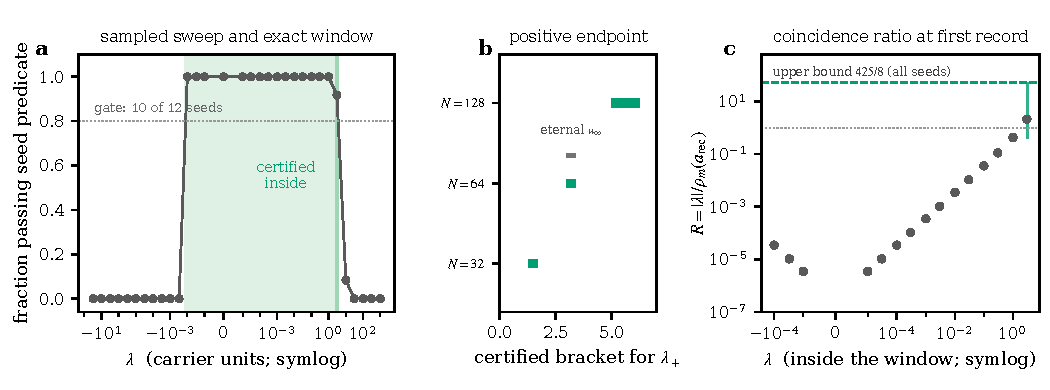
\includegraphics[width=\textwidth]{F3_window.pdf}
\caption{\textbf{The record window.} \emph{(a)} Fraction of the twelve seeds passing the both-tag seed predicate in the
original sampled sweep (grey). The admitted window is $(-1/8000,\lambda_+]$: the light green region $(-1/8000,3]$ is
certified to lie inside it, and the darker band is the certified bracket $3<\lambda_+<3.4$ for its upper edge. \emph{(b)} Certified brackets for the upper edge of the three separately realized populations, and for
the eternal-record edge $u_\infty$ of the 64-patch population. \emph{(c)} Seed-median coincidence ratio at the first
record in the sampled sweep (grey) with the certified bounds: $R<425/8$ throughout the window for every seed (dashed) and
$3/8<R(\lambda_+)<425/8$ at the upper edge (green box; its horizontal extent is the bracket for $\lambda_+$). The ratio can also be made arbitrarily small at admitted
$\lambda>0$.}
\label{fig:window}
\end{figure}
